%----------------------------------------------------------------------------------------
%	PACKAGES AND OTHER DOCUMENT CONFIGURATIONS
%----------------------------------------------------------------------------------------

\documentclass[10pt]{article}											% font size

\usepackage{myStyle}													% Use a custom style sheet: double column, police, text...
\usepackage{subfig}
\usepackage{graphicx}													% to include images
\usepackage{float}														% to float figures
\usepackage{booktabs,makecell}											% for diagonal cells
\usepackage{hyperref}													% for hyperlinks
\usepackage{listings}													% for including files
%\usepackage[top=1in, bottom=1in, left=1.25in, right=1.25in]{geometry}	% set margins
\usepackage[top=0.75in, bottom=0.70in, left=0.70in, right=0.70in]{geometry}	% set margins
\usepackage[utf8]{inputenc}												% for unicode input characters
\usepackage{helvet}														% use helvetica per default
\usepackage[T1]{fontenc}
\usepackage[english]{babel}
\usepackage{multicol}													% To make the document with many columns

\setlength{\columnsep}{1cm}
\renewcommand{\familydefault}{\sfdefault}								% use sans serif per default

\lstset
{
  basicstyle=\scriptsize\sffamily,%
  commentstyle=\footnotesize\ttfamily,%
  frameround=trBL,
  frame=single,
  breaklines=true,
  showstringspaces=false,
  numbers=left,
  numberstyle=\tiny,
  numbersep=10pt,
  keywordstyle=\bf
}


%----------------------------------------------------------------------------------------
%	TITLE SECTION 
%----------------------------------------------------------------------------------------

\makeatletter
\makeatother
\renewcommand{\familydefault}{\sfdefault} % use sans serif per default
\makeatother

\begin{document}

\title{Impact of memory allocation on the performance of a delegation synchronization algorithm}
\author{Written by Riyane SID-LAKHDAR (M1 MoSIG)\\
Supervised by Thomas ROPARS (LIG, team ERODS)}
\maketitle




%----------------------------------------------------------------------------------------
%	ABSTRACT
%----------------------------------------------------------------------------------------



%****************************** TODO\\
% Trouver des synonimes a performance issue: downgrading/drop/reduction/decline/deterioration/ 
%********************* End TODO

\begin{abstract}
%- ******Context\\
Memory allocation is a complex operation that can have a deep impact on the performance of concurrent algorithms.   Delegation represents an example of such algorithms.   However, few studies have been conducted to assess such an impact.
%Concurrent programming techniques use the dynamic memory as a simple way to synchronize concurrent threads.   Thus memory allocation has an obvious impact on the performance of  distributed algorithms.   Delegation is a thread synchronization technique that illustrates well such an impact.


%- ******problems\\


%- ******Results\\
This paper exposes our evaluation of two delegation algorithms with state of the art allocators on two multicore platforms.

%- ******Conclusion\\
We show that the used allocator may limit the performance of the considered multithread applications.   We also demonstrate that the delegation algorithm performing best depends on the allocator performance and the considered hardware architecture.

\end{abstract}

%****************************** TODO\\
%	- Modifier imperativement les tittres (AHHHHHHH)\\
%    - Verifier les temps et les formes des tittres (passives/actives)\\
%*********************** End TODO


%----------------------------------------------------------------------------------------
%	INTRODUCTION
%----------------------------------------------------------------------------------------
\section{Introduction}
With the rise of many-core processors, concurrent programs have increased the efficiency of existing algorithms by simply splitting their tasks over concurrent cores.   However, due to hardware and software issues, parallelizing the execution of a task using \textit{N} cores does not mean dividing its execution time by \textit{N}.\\

Among the things that can limit the efficiency of concurrent algorithms, memory allocation is one that is often disregarded but that can still deeply affect performance. The main problem when dealing with a large number of threads,  that frequently allocate and free memory, is that the memory allocation system may receive requests from different threads at the same time.   If the memory allocation system answers the requests sequentially, it becomes the performance bottleneck of multithreading ~\cite{cacheCoherence_sorin}.\\

Another issue for multithreaded applications is the need to synchronizing concurrent memory accesses ~\cite{cacheCoherence_sorin}.   In this context, \textit{delegation} ~\cite{delegationCS_roparsPetrovic} is an example of contributions to implement efficiently mutual exclusion on shared objects.   However, existing evaluations of \textit{delegation} algorithms have been obtained using a custom allocator \footnote{Allocator that outperforms the time efficiency of general-purpose allocators by using a relatively large and thread local dynamic memory.   Hence, such an allocator cannot be used as a general-purpose one.}.   Hence our main objective is to study how delegation algorithms would perform when used with state-of-the-art general-purpose allocators.\\

Different strategies have been proposed to improve the efficiency of dynamic memory management.   Thus, in the present work, we first introduce, in section \ref{stateOfTheArtAllocator}, an overview of the main state-of-the-art allocators for multithreaded systems.

Section \ref{experimentalSetup} and \ref{results} present our experimental evaluation of two custom \textit{delegation} algorithms over two specific processor architectures:  a 20 cores Intel Sandy Bridge, and a 24 cores AMD Bulldozer.\\

Using \textit{tcmalloc}, the allocator implementation that best fits our workbench, we are able to infirm some properties previously obtained on the considered AMD architecture.   Thus the impact of memory allocation on shared memory algorithms is clearly highlighted.


%----------------------------------------------------------------------------------------
%	CONTEXT AND MOTIVATION
%----------------------------------------------------------------------------------------

\section{Context and motivation}
Any application that tries to dynamically manage memory on a \emph{NUMA} multicore system faces a set of issues that impact its performance.   In this section, we highlight these issues.   We also explain how the complexity and the heterogeneity of these challenges motivate the need beneath the comparison of allocators: an inefficient allocator may dramatically influence the evaluation of thread-synchronization mechanisms.


%----------------------------------------------------------------------------------------

\subsection{Complex processor architecture}
Let us consider a \textit{Non Uniform Memory Access (NUMA)} processor (see Figure \ref{globalNumaArchitecture.png}).   To maintain a set of data coherent and up-to-date over such an architecture, an important time and space overhead is required.   Indeed, this architecture represents a complex structure with several levels of caches which need to stay coherent ~\cite{cacheCoherence_sorin}.   Coherence property has to hold despite the different cores accessing the caches asynchronously.\\

	\begin{figure}
		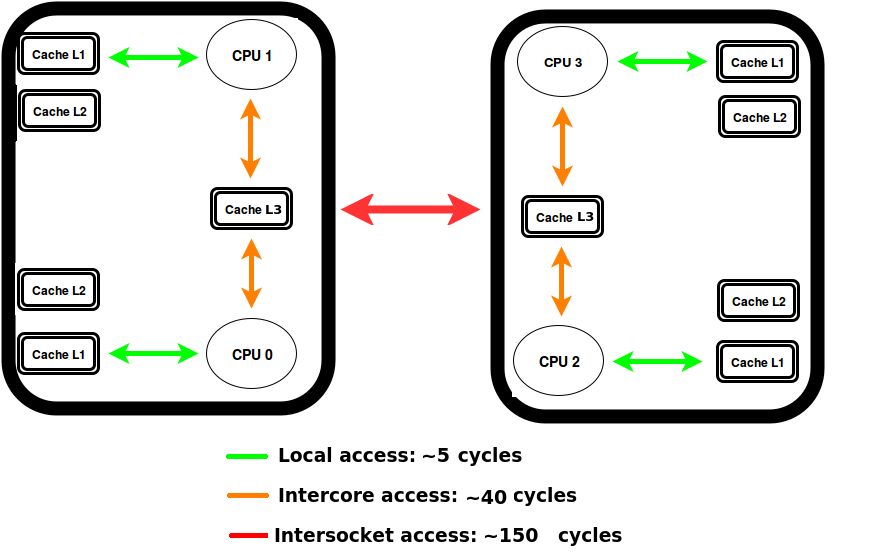
\includegraphics[width=1.0\linewidth]{charts/numaNode.png}
		\caption{Simplified NUMA model and latency on \textit{Intel Sandy Bridge} architecture}
        \label{globalNumaArchitecture.png}
	\end{figure}

The multicore processor architecture that we consider (NUMA) are made of multiple components interconnected by a network-on-chip.   Thus, any interaction between two independent components involves network communication which, in turn, induce a non negligible overhead.\\
When a thread tries to reach an address kept by its current L1 cache, the access may be done in a relatively short time (about 2 CPU cycles).   However, this value may dramatically increase when the address is kept by a foreign core:  up to 40 CPU cycles when the core is on the same NUMA node (L3 cache) and 150 CPU cycles when the core is on a foreign node (socket communication).


%----------------------------------------------------------------------------------------

\subsection{False sharing, memory blowup and heavy kernel operations}
The allocation and the liberation of dynamic memory is unpredictable and asynchronous\cite{cacheCoherence_sorin}.   Thus, after a period of time, any set of dynamically-used memory may become fragmented:   relatively small blocks of free and used memory are highly interleaved.\\
Dealing with a fragmented memory may impact the allocation performance:   When the user requires a given block of memory, the allocator may have no free chunk of memory large enough to satisfy the request, while the total free memory may still be enough.   Depending on the allocator implementation, the request may remain unsatisfied, or the process heap may be dynamically expanded.   But in all cases a non negligible delay is appended to the allocation time.   This performance deterioration is known as \textbf{\textit{memory blowup}}.\\

	\begin{figure}
				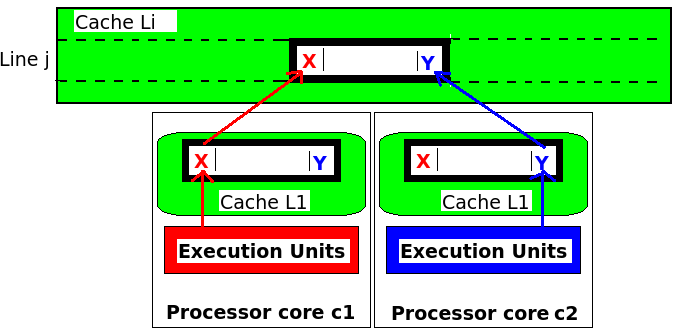
\includegraphics[width=1.0\linewidth]{charts/falseSharing.png}
		\caption{False sharing representation}
		\label{falseSharing.png}
	\end{figure}

Another performance drop, known as \textbf{\textit{false sharing}}\cite{hoard_berger} may appear at access time.   Let us consider two separate objects accessed by two different threads running concurrently on two different cores.   Let us also suppose that the two objects are stored in the same cache line (see Figure \ref{falseSharing.png}).   As these objects have different address ranges, they could safely be accessed simultaneously.   However, as the access granularity in the cache is a cache line (typically 64 Bytes), the cache controller will execute these accesses sequentially, increasing thus the total access time.\\

Finally, the memory is a resource shared by independent processes running on separate cores.   For memory coherence reasons, managing this memory must be done at kernel level.   Thus, any memory allocator is subjected to the use of a set of heavy operations, often involving system calls.


%----------------------------------------------------------------------------------------

\subsection{Testing a new algorithmic approach: Delegation for mutual exclusion}
Our paper follows the work of \textit{D. Petrovic}, \textit{T. Ropars} and \textit{A. Schiper} ~\cite{delegationCS_roparsPetrovic}.   In this former paper, an algorithm, based on the \textbf{\textit{delegation approach}} to implement mutual exclusion is described (see Section \ref{delegationSynchronizationAlgo_description}).   This algorithm is experimentally shown to achieve "1.4x (resp. 2x) higher throughput compared to the most efficient state-of-the-art delegation solution" ~\cite{delegationCS_roparsPetrovic}.\\

One limitation of this study is that the experimental tests of the algorithms have been conducted using a \textit{custom allocator}, built in order to allocate and free memory in short and roughly constant time.   The principle of this allocator is to pin to each thread a block of memory at creation time.   The dynamic memory management is optimized by always allocating fix-sized chunks from this block.   No address of this block is freed until the thread destruction.   As such, this allocator is ideal for this study.   However, it can not be used for general purpose applications.\\

Regarding the wide scope and the complexity of the challenges associated with dynamic memory allocation, one can wonder how the use of a \textit{general-purpose allocator} could affect the performance and behavior of the delegation algorithms.   To answer this question, we need to identify the most suitable general-purpose allocator for our workload.






%----------------------------------------------------------------------------------------
%	STATE OF THE ART
%----------------------------------------------------------------------------------------

\section{State of the art}\label{stateOfTheArtAllocator}
As many-core machines have become widely used, different memory allocators ~\cite{glibc_robertson,hoard_berger,scalloc_aigner,supermalloc_kuszmaul,jemalloc_evans,tcmalloc_ghemawat} have been proposed to try to fit the needs of this programming paradigm.   Each of these implementations has either proposed some new memory-allocation strategies or has improved an existing one.   In this section, we give an overview of some of these strategies.  We highlight their advantages and link them to some existing implementations.


%----------------------------------------------------------------------------------------

\subsection{Delegate memory allocation to user space program}
Among the set of functions that an operating system (OS) proposes to a user program, the ones that trigger a system call are probably the costlier in terms of time (only considering the non blocking instructions).   They imply a switch to kernel mode, increasing the execution time of the task.\\

In the \textit{Linux OS} C standard library \textbf{\textit{glibc}} ~\cite{glibc_robertson}, the memory-allocation function regularly re-sizes a process heap at runtime.  Thus, allocation functions may trigger system calls\footnote{Call to the kernel functions \textit{brk}, \textit{sbrk} and \textit{mmap}}.   To decrease to almost zero the number of these system calls, all the memory allocators that we will consider use the same strategy: a large chunk of memory is initially allocated to all user programs.   Allocation is then done at user level by simply splitting this initial chunk of memory.

This method dramatically decreases the number of system calls.  Yet, when the initially-allocated memory is exceeded, user allocators may trigger a system call to seek the OS for a new chunk of memory (as in \textbf{\textit{Hoard}} ~\cite{hoard_berger}, \textit{\textbf{tcmalloc}} ~\cite{tcmalloc_ghemawat} or \textbf{\textit{SuperMalloc}} ~\cite{supermalloc_kuszmaul}) or to answer each new allocation request made by the user (as in \textit{Scalloc} ~\cite{scalloc_aigner}).


%----------------------------------------------------------------------------------------

\subsection{Core locality allocation}
Within \textit{UNIX} processes, process heap is a resource shared by many threads.   Thus, to ensure consistency, synchronization is required between threads that try to access it, which obviously introduces a time override.\\

To decrease this synchronization override, \textbf{\textit{Hoard}} ~\cite{hoard_berger}, which is one of the first thread-scalable allocators, has introduced the idea of core locality:  each processor core is mapped to a unique buffer. Threads running on this core are the only one authorized to allocate memory in this buffer. Hence, allocation requires no synchronization between threads from different cores.   \textbf{\textit{tcmalloc}} uses an adaptation of this method where a buffer is mapped to each thread.   The core local principle has been further improved by \textbf{\textit{Scalloc}} ~\cite{scalloc_aigner} by adapting the data structure used for the buffer (see Section \ref{virtualSpanDefinition})\\

One of the main advantages of the core local buffer is the increasing probability that a thread triggers a page fault.   Indeed, a buffer is allocated as a block of contiguous addresses.   All the threads running on a given core allocate memory within the same address range (addresses of the buffer).   Thus the probability to trigger a page fault is low, even after a context switch.


%----------------------------------------------------------------------------------------

\subsection{Dealing with the shared pool contention}
To feed each core-mapped buffer, an allocator may reuse a freed memory previously belonging to the same buffer (with no synchronization over-cost).   It also needs a structure supplying an empty buffer request (see Figure \ref{globalArchitecture.png}).\\
This structure is made of one stack per core.  Hence, it may be safely accessed by all the core-local buffers simultaneously and without any synchronization.\\

\begin{figure}[H]
    \centering
    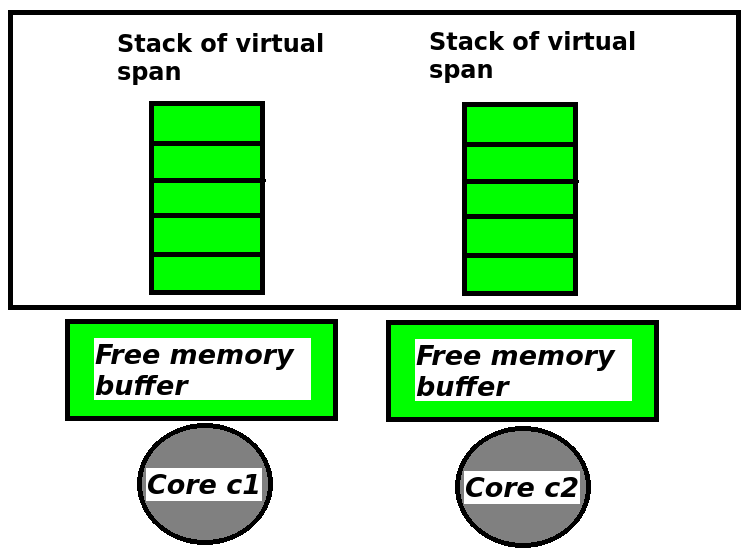
\includegraphics[width=0.4\textwidth]{charts/globalArchitecture.png}
    \caption[Caption for FN]{Free memory pool: shared by all the cores. \emph{TLAB}: Thread Local Allocation Buffer}
    \label{globalArchitecture.png}
\end{figure}

One important efficiency factor of this shared structure is the number of requests it makes to the OS kernel to get more free memory.   To reduce this number, the policy introduced by \textbf{\textit{supermalloc}} ~\cite{supermalloc_kuszmaul} is to maintain the fill rate of all the core-mapped stacks roughly equal.   The OS kernel requests are only made once the average level of the stacks reaches a given threshold value.\\
Using such a policy, a core-mapped stack that runs out of memory will very likely be filled from another stack.  Contention on the core-mapped stacks has been lightened by \textbf{\textit{scalloc}} ~\cite{scalloc_aigner} through the usage of the non blocking \textit{Treiber stack} ~\cite{treiberStack}.   Similarly, \textbf{\textit{tcmalloc}} uses a lock-free multilevel linked list.\\

These strategies have made it possible to remove almost all synchronization for allocation operations, making them having a roughly constant number of micro instructions.   However, a chunk of memory allocated by a given thread may be freed by a different one.   Thus, to avoid a synchronization over-cost for the \textit{free} operation, \textbf{\textit{scalloc}} ~\cite{scalloc_aigner} does not return a freed memory to the shared pool.  It places it instead into the buffer of the thread which runs the \textit{free} function.


%----------------------------------------------------------------------------------------

\subsection{Virtual span} \label{virtualSpanDefinition}
So far, we have considered solutions that improve the efficiency of memory management by adapting the \textit{allocation} and \textit{free} operations.   Further improvements can be obtained by reducing the access time to a given address.

Within \textbf{\textit{scalloc}} ~\cite{scalloc_aigner}, \textbf{\textit{jemalloc}} ~\cite{jemalloc_evans} and \textbf{\textit{tcmalloc}} ~\cite{tcmalloc_ghemawat} , the free memory is organized using the principle of so-called \emph{virtual span}\footnote{Also called \emph{superblock} (resp \emph{superpage}) for \emph{Hoard} ~\cite{hoard_berger} (resp \emph{jemalloc} ~\cite{jemalloc_evans}) implementation.}.   This structure consists of a fixed-size block of contiguous addresses.   Nine different size classes exist (), each of them is a multiple of 4KB (the size of a system page).   An allocation results in the use of one independent span, no matter the size required by the user. 
The payload of the object is stored into the span.   Additionally, some extra memory is used for alignment and uniformity purposes.\\

This architecture has been designed to improve \emph{space locality}, avoid \emph{fragmentation} and simplify \emph{complex data structures} \footnote{\emph{False sharing} is also dramatically reduced thanks to the virtual span.   An experimental evaluation of this improvement is available in ~\cite{scalloc_aigner}}.


%----------------------------------------------------------------------------------------

\subsubsection{Space locality}
The operating systems that we are considering implement \emph{virtual paging}.   Thus, a major concern for time efficiency is that memory addresses, which are more likely to be used together, may belong to the same page.   This property reduces the number of page faults, which is a major time consuming factor.\\
As a virtual span is a set of contiguous addresses, it increases the probability that two addresses of the same object (allocated by the same call to the “allocation” function) belong to the same page.


%----------------------------------------------------------------------------------------

\subsubsection{Fragmentation and complex data structures}
Storing exclusively a few number of size-range objects has an obvious interest for avoiding fragmentation and simplifying data structures used for management.   On the other hand, as we treat uniformly large and small objects, an important extra memory may be required for small objects.   However, thanks to the paging system, this unused memory is swapped out of the live memory (RAM) and will never trigger a page fault (never accessed by the user).   Thus, the pagination system limits the time and space impact of the extra memory used by a span.


%----------------------------------------------------------------------------------------
%\subsection{Face memory blowup}
%\subsection{garbage collection}
%**********TODO**************








%----------------------------------------------------------------------------------------
%	EXPERIMENTAL SETUP
%----------------------------------------------------------------------------------------

\section{Experimental setup}\label{experimentalSetup}
It is noteworthy that the results of our experiments are highly dependent on the processor architecture and the operating\\
In this section, we explicitly define the hardware and software environment used to obtain the presented results.   We also define the algorithm that we aim to evaluate, as well as the rules of the evaluation.\\

\subsection{Custom delegation algorithms for synchronization}\label{delegationSynchronizationAlgo_description}
The algorithms we want to evaluate ~\cite{delegationCS_roparsPetrovic} implement a critical section using the \emph{delegation} principle: given a critical section CS, each thread that tries to access it will send a request to a dedicated centralized thread (server).   The server will answer the requests sequentially, by being the only one to access (and realize) the CS.\\

The first considered delegation algorithm is the \textbf{\textit{combiner algorithm}}.  In this algorithm, the server thread is not a specific dedicated one.   Indeed, when different client threads try to access a CS, one of these threads is elected to execute its own CS as well as the one of a certain number of other threads.\\


The other considered algorithm implements two main improvements to the delegation method.   The first one consists in the use of a \textbf{\textit{back-off}} on client side in order to reduce the overhead due to a remote memory reference:
Let us consider a client thread that has written a request to the server, and which spins on a specific memory address M, waiting for the answer.   The first improvement consists in adjusting this spinning rate to the \textit{prefetcher} rate, in order to delay the first read access of the client.   Thus, we increase the probability that the server accesses the CS between the client's write and the first client's read.   As the server holds a \emph{read write} access on M during this period, it may write the answer without updating the client's cache.   Hence avoiding the server to trigger a costly remote memory reference to the client. 

The second improvement consists in using a non-temporal memory access (\textbf{\textit{Streaming store}}) for the communication between the clients and the server.   Therefore, the server avoids waiting for the write operation to be effective.


%----------------------------------------------------------------------------------------

\subsection{Hardware and software environment}
The results that are presented in this paper have been obtained on two x86 machines (accessed through the test-bed \textit{Grid5000}).   The first one is an \textit{Dell Poweredge C6220} consisting of two 10-core \textit{Intel Xeon E5-2660v2} (2.2GHz) chips.   The second one is an \textit{HP Proliant DL165 G7} consisting of two 12-core \textit{AMD Opteron 6164 HE} (1.7 GHz) chips.\\
On both machines, a linux (3.16.7-4) operating system has been used based on the Debian kernel 3.16.7.   The default kernel allocation policy (first touch) has been used to obtain all the presented results.\\
All the programs that implement the CS algorithms and the shared data structures have been implemented in C language.   They have been compiled using \textit{gcc 4.4.7}.  The option O3 (maximum optimization level) has been used for all the compilation process.\\

For the experiments, the following memory allocators have been considered : \emph{glibc} 3.74, \emph{Hoard} v2.2.1, \emph{scalloc} (released in August 2015), \emph{Supermalloc} (released in June 2015), \emph{gperftool-tcmalloc} v 3.2.1 and \emph{jemalloc} 4.2.1. 


%----------------------------------------------------------------------------------------

\subsection{Testing environment and rules}

The experimentation that we lead have all been conducted using applications built on the same principle:  A fixed number of threads concurrently access a queue.   The queue is a \emph{Michael Scott queue} ~\cite{queue_michaelScott} synchronized using one of the presented CS delegation algorithms.   Each thread loops on the \textit{enqueue} and \textit{dequeue} actions.   Each appended/removed element is allocated/freed dynamically. 

Our implementation ensures that:
\begin{itemize}
	\item Each application uses less threads than the number of cores available on the machine.   This constraint helps in lightening the waiting time due to scheduling.
	\item Each thread is pinned to a distinct core.   This constraint eliminates the cost of reaching an address owned by a cache within another core.   It also eliminates the OS scheduler inference on the performance.
\end{itemize}







%----------------------------------------------------------------------------------------
%	RESULTS
%----------------------------------------------------------------------------------------
\section{Results}\label{results}
In this section we use the \textit{throughput} (number of queue access operations per second) as metric for our comparative study.   Other metrics, such as the \textit{latency} or the \textit{inter-core fairness}, have been considered.   However, they have been omitted on purpose in this paper as they did not add any significant value to the study.\\


%----------------------------------------------------------------------------------------

\subsection{Choosing the most efficient memory allocator}\label{allocatorComparison}
First, we evaluate the impact of the memory allocator on the throughput of our test application. In the current case, the shared queue is implemented using the \emph{combiner algorithm}.   Figure \ref{allocatorComparison.png} shows the throughput of this application when different allocators are used.

\begin{figure*}[t]
\begin{center}
	\subfloat[Intel Xeon E5 2620]
    {
		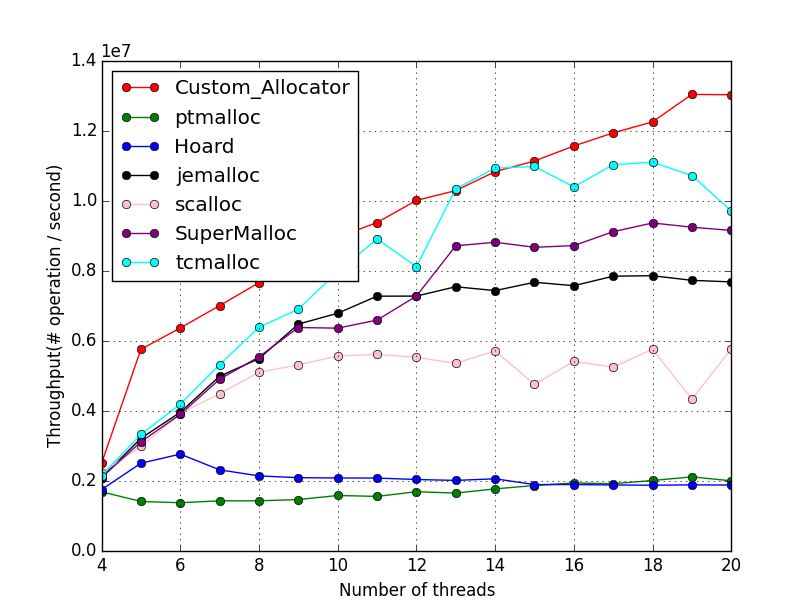
\includegraphics[width=0.4\hsize]{charts_allocator/20-Intel_Xeon_E5_2620-noOption-0-cc-msqueue.png}
	}
	\subfloat[AMD Opteron 6164 HE]
    {
		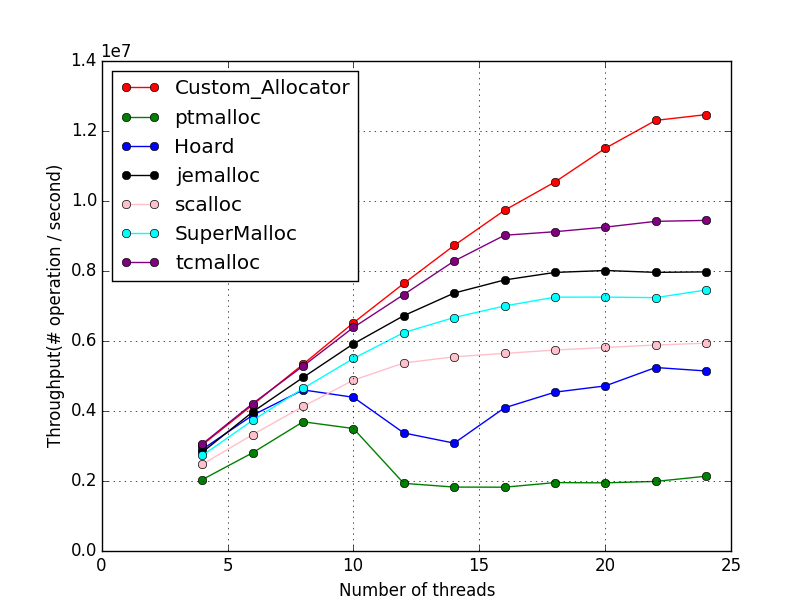
\includegraphics[width=0.4\hsize]{charts_allocator/24-AMD_Opteron_6164_HE-noOption-0-cc-msqueue.png}
	}
	\caption{Impact of the memory allocator on the performance of multithreaded application}
	\label{allocatorComparison.png}
\end{center}
\end{figure*}


We can notice in this figure three main groups of allocators, gathered according to their performances:\\
On one hand, the \textit{custom} allocator which, as expected, outperforms  all the others from $20\%$ up to $530\%$.   Respectively, the \emph{ptmalloc} allocator underperforms all the allocators from $100\%$ up to $500\%$.  On the other hand, the general purpose allocator may be sorted according to their implemented strategies:
\begin{itemize}
	\item \textit{Hoard}, which only implements the core local buffer, is the least efficient one.   It has also the least stable behavior due to the non reuse of the freed memory: after a given period of time, the core local buffers get empty, and a system call (sequential) is required to feed them.   As the importance of this phenomenon increases with the number of concurrent threads, this explains the dramatic drop of the \textit{Hoards}'s curve after 10 threads.

	\item \textit{SuperMalloc, scalloc} and \textit{jemalloc} may be considered as equivalent.   The difference that can be observed in their curves are due to the management of the released memory.   Indeed, \textit{jemalloc} places it into the core local buffer with no synchronization (one thread per core); whereas \textit{SuperMalloc} and \textit{scalloc} place the released memory into the shared pool which requires a synchronization with the other threads on the other cores.

	\item Similarly to the previous allocators, \textit{tcmalloc} uses a thread local buffer and a shared free data structure.    The efficiency gain that we notice comes from the use of a \textit{garbage collector}:  Thanks to this asynchronous and T periodic feature, the free operation is equivalent to a simple boolean variable modification.   The overhead linked to the free operation is payed only once at each period T.
\end{itemize}


%----------------------------------------------------------------------------------------

\subsection{Custom delegation algorithm performance using a real allocator}
Thanks to the previous experimental results, we can definitely choose \textit{tcmalloc} as an allocator for the benchmark study of the considered delegation algorithms.

Using this allocator, we present in Figure \ref{delegationAlgorithmComparison.png} the performance comparison of a shared queue implemented using each of the considered delegation algorithms.\\

\begin{figure*}[t]
\begin{center}
	\subfloat[Intel Xeon E5 2620]
    {
		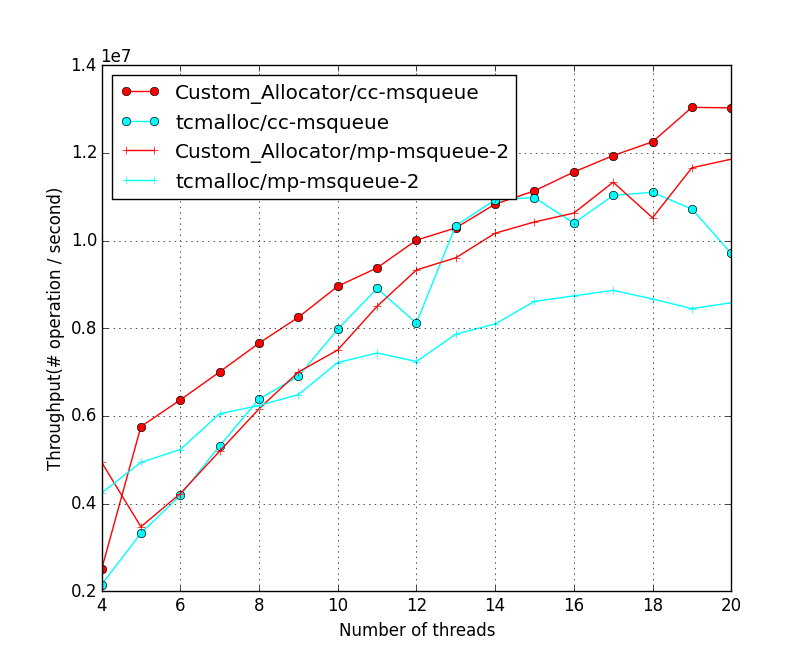
\includegraphics[width=0.4\hsize]{charts_allocator/20-Intel_Xeon_E5_2620-noOption-0-cc-msqueue+350-mp-msqueue-2-tcmalloc+Custom_Allocator.png}
	}
	\subfloat[AMD Opteron 6164 HE]
    {
		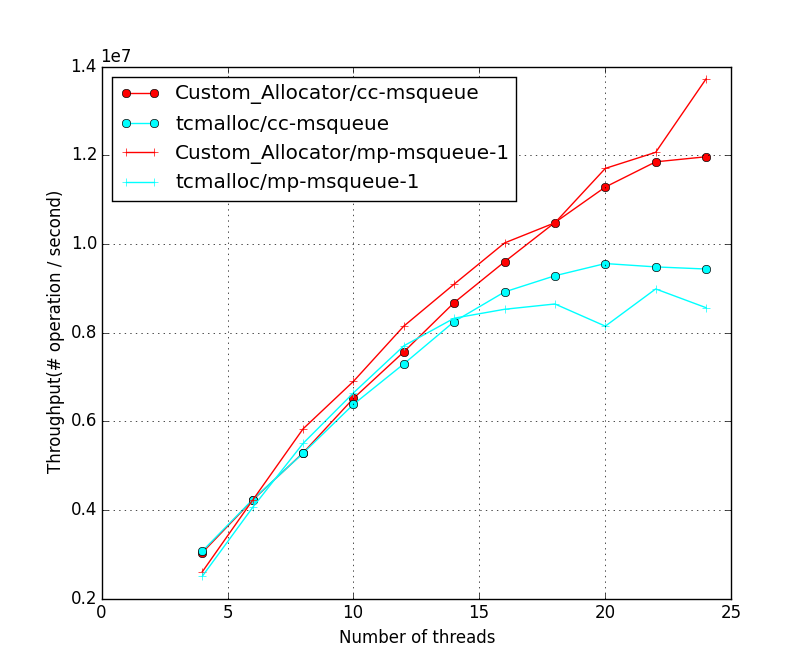
\includegraphics[width=0.4\hsize]{charts_allocator/24-AMD_Opteron_6164_HE-noOption-0-cc-msqueue+400-mp-msqueue-1-tcmalloc+CustomAllocator.png}
	}
	\caption{Delegation algorithm comparison using the tcmalloc allocator. Custom-Allocator used as a benchmark.   \emph{cc-msqueue}:  shared queue implemented using the combiner algorithm.   \emph{mp-msqueue-2}: shared queue implemented using the backoff/streaming delegation algorithm}
	\label{delegationAlgorithmComparison.png}
\end{center}
\end{figure*}

Our method confirmed the results obtained by \emph{D. Petrovic et al} ~\cite{delegationCS_roparsPetrovic} on the considered Intel architecture.   The optimized delegation algorithm reaches, in this specific condition, a higher throughput than the \emph{combiner} algorithm (about 10\%).  And this result holds using both \textit{custom} and \textit{tcmalloc} allocators.

However, our experimental results infirm the claim of \emph{D. Petrovic et al} ~\cite{delegationCS_roparsPetrovic} on the considered AMD architecture.   Indeed, within this specific conditions, the combiner algorithm reaches a higher throughput.\\


%----------------------------------------------------------------------------------------

\subsection{Discussion}
From our experimental results, two noteworthy results may come out.   On one hand, the experimental comparison of the allocators shows the highly significant difference between the custom allocator used in the former test of the delegation algorithm, and the general purpose allocators.   It also shows how stable is the behavior of this custom allocator compared to the others.   This justifies the need of the current benchmarking study in order to validate any performance property of the custom delegation algorithms.\\

On the other hand, all the conclusions that come out of our experimental results are intrinsically dependent on the two considered hardware platforms and kernel policies.   Indeed, the comparison between our experiments and the one conducted by \textit{D. Petrovic et al} shows an obvious difference between the maximum threshold performance reached by the same algorithm (considering the same number of threads).   Such a difference may be principally explained by the different number of NUMA nodes used during the two experiments:  the highest is the number of NUMA nodes, the more the hosted application triggers costly remote memory references.

%Yet, this throughput difference highlights an important aspect of our study:   all the conclusions that come out of our experimental results are highly dependent of the two considered hardware platforms and kernel policies.   Despite of the remarkable similarity between our hardware platform and the one used by \emph{D. Petrovic et al}, the comparison and the link between the two studies is intrinsically dependent of this hardware difference.
%In an other hand, it is interesting to notice that during our experiments, we have reached a maximum throughput of 11M (resp. 9.7M) operations on the considered Intel (resp. AMD) architecture using only 20 (respectively 24) hardware threads.   At the same time, the experimental results of \emph{D. Petrovic et al} have barely reached the same threshold throughput using 40 (respectively 25) hardware threads.   Such a performance threshold difference is due to the number of NUMA nodes which is much higher in the environment considered by \textit{D. Petrovic et al}:  the highest is the number of NUMA nodes, the more the hosted application triggers costly remote memory references.\\
%As the measured latency per core is relatively weak, such a throughput difference may also be due to the difference between the core frequencies (lower in the environment of \textit{D. Petrovic et al}).\\
%The noticed difference in hardware capacity highlights an important aspect of our study:   all the conclusions that come out of our experimental results are highly dependent of the two considered hardware platforms and kernel policies.   Despite of the remarkable similarity between our hardware platform and the one used by \emph{D. Petrovic et al}, the comparison and the link between the two studies is intrinsically dependent of this hardware difference.



%----------------------------------------------------------------------------------------
%	CONCLUSION / DISCUSSION
%----------------------------------------------------------------------------------------
\section{Conclusion}

The current paper presents our method to prove the impact of memory allocation on the performance of two custom delegation algorithms.   Our evaluation shows that such an impact does not corrupt the expected behavior of the delegation algorithms.   However, we have proved that depending on the considered platform , the validation of an improvement of the delegation approach may go on default.




%----------------------------------------------------------------------------------------
%	REFERENCES
%----------------------------------------------------------------------------------------
\nocite{*}
\small{\bibliographystyle{abbrv}
\bibliography{bibliography.bib}\vspace{0.75in}}


\end{document}